\chapter{Wytrenowanie bota}
\thispagestyle{chapterBeginStyle}

\subsection{Cel i funkcjonalności}
Wytrenowany bot powinien być w stanie poruszać się po wygenerowanym wcześniej terenie, rozpoznając i trzymając się drogi. Trening bota powinien wykorzystywać metody uczenia przez wzmacnianie.

\subsection{Wykorzystane technologie}
Silnik Unity udostępnia dodatek open-source ML-Agents \cite{UnityMlAgentsRepository} \cite{UnityMlAgents}, który pozwala na wykorzystanie środowisk utworzonych w grze do treningu modeli. Stanowi on warstwę łączącą Unity z biblioteką Tensorflow, oraz zapewnia wiele nowoczesnych algorytmów głębokiego uczenia przez wzmacnianie (m.in. Proximal Policy Optimization (PPO), Soft Actor-Critic (SAC), self-play). W powyższej pracy wykorzystano algorytm PPO, ze względu na większą stabilność treningu \cite{CompareDrlAlgorithms}. Śledzenie wielu metryk postępu uczenia było dostępnych z wykorzystaniem programu tensorboard.

\subsection{Uczenie przez wzmacnianie}
Uczenie przez wzmacnianie jestem jednym z trzech głównych nurtów uczenia maszynowego, gdzie agent uczy się polityki optymalnej w danym środowisku metodą prób i błędów, otrzymując wyłącznie wartość nagrody jako informację zwrotną. W przeciwieństwie do uczenia nadzorowanego, metoda ta nie wymaga wcześniejszego przygotowania dużej ilości opisanych danych. Pozwala to na wprowadzenie bota do nieznanego środowiska i natychmiastowe podjęcie interakcji.\\
Cykl uczenia przez wzmacnianie opiera się na akcji bota i reakcji. Bot zbiera obserwacje na podstawie stanu w jakim się znajduje w środowisku. Następnie podejmuje decyzję na podstawie obserwacji. Po podjęciu decyzji wykonywana jest odpowiednia akcja, po czym za akcję przyznawana jest nagroda lub kara, w zależności czy akcja wpłynęła pozytywnie na przybliżanie się bota do celu. Na podstawie zbioru informacji zawierającego stan początkowy, podjęte akcje i otrzymaną nagrodę trenowana jest polityka, maksymalizując oczekiwaną nagrodę.
\clearpage
\subsection{Metodyka uczenia}
Wstępne uczenie odbywa się na terenach płaskich (wysokość każdego punktu jest równa zero) oraz w terenie ze zwiększonym kontrastem - droga jest czarna a wszystko pozostałe jest białe. Do treningu uruchomione jest naraz 12 terenów, zawierających 4 różne trasy. Na każdym z terenów znajduje się pomiędzy 1 a 4 pojazdy, co oznacza że model jest trenowany na 12-48 niezależnych instancjach naraz, w celu przyspieszenia nauki. W kolejnych etapach zwiększany jest stopień trudności trasy, reprezentowany przez ilość i ostrość zakrętów. Następnie zwiększane jest pofałdowanie terenu, oraz zmieniane są tekstury drogi i terenu.
\begin{figure}[H]
    \centering
    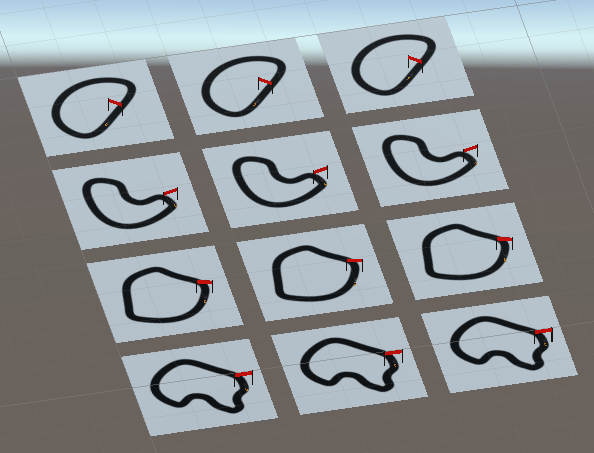
\includegraphics[width=.5\textwidth]{figures/multiple_tests}
    \caption{Prowadzenie wielu treningów na raz}
    \label{fig}
\end{figure}

\subsection{Analiza wyników}
Wyniki uczenia przedstawione zostały na wykresie za pomocą dwóch metryk. Wartość \textit{Cumulative Reward} oznacza średnią wartość nagrody z jednego epizodu dla jednego agenta. Wartosć \textit{Visited punkt kontrolnys} informuje jak dużą część trasy przeszedł agent, uśrednioną z jednego epizodu dla jednego agenta. Pełne okrążenie zaweira w sobie 40 punktów kontrolnych. Wartości zaznaczone na wykresach bledszym kolorem są wartościami rzeczywistymi, natomiast wartości pogrubione wyliczone zostały z wykorzystaniem średniej kroczącej eksponencjalnej, aby lepiej uwidocznić tendencje zmian.

\begin{figure}[H]
    \centering
    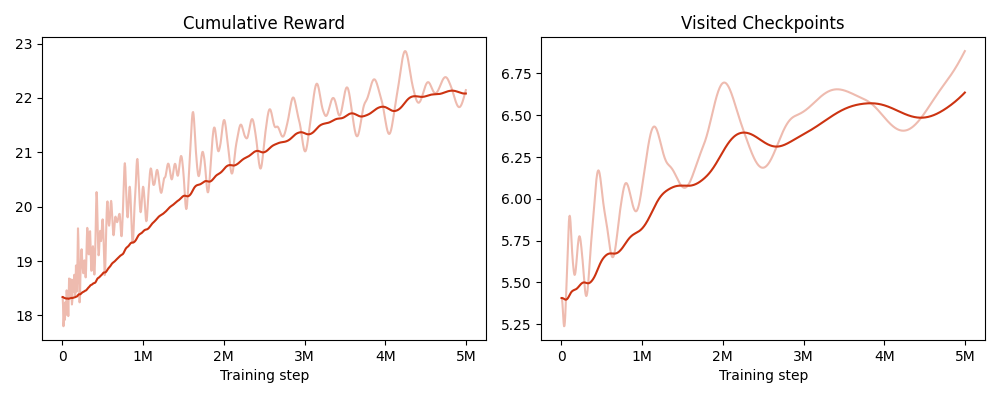
\includegraphics[width=\textwidth]{graphs/example}
    \caption{Przykładowa analiza wyników}
    \label{fig}
\end{figure}

\subsection{Wybór obserwacji}
Wybór informacji, jakie dostępne są dla bota znacznie wpłynie na podejmowane przez niego decyzje. Za mała ilość informacji nie pozwoli na wykrycie odpowiedniej ilości szczegółów trasy, natomiast za duża znacznie zwiększy czas treningu i inferencji, wprowadzając niepotrzebny szum.

\subsubsection{Dane wynikające z trasy}
Pierwszy sposób obserwacji opiera się na wartościach, do których zwykły gracz nie ma dostępu, ponieważ wymagają m.in. znajomości dokładnego wzoru  krzywej trasy do wyliczenia. Dane, które są przekazywane do modelu jako obserwacje to:
\begin{itemize}
    \item odległość w linii prostej od aktualnej pozycji do centrum szerokości trasy
    \item kąt pomiędzy kierunkiem jazdy pojazdu a kierunkiem stycznej do toru
    \item odległość w linii prostej od aktualnej pozycji do najbliższego punktu kontrolnego
    \item kąt pomiędzy kierunkiem jazdy pojazdu a kierunkiem do najbliższego punktu kontrolnego
    \item kąt nachylenia terenu
    \item aktualna pozycja kół ($-1$ oznacza maksymalnie skręcone w lewo, $1$ maksymalnie w prawo)
    \item aktualny stopień wciśnięcia pedału gazu ($-1$ oznacza jazdę do tyłu, $1$ jazdę do przodu)
    \item aktualna prędkość
\end{itemize}

\subsubsection{Dane odległości od krawędzi}
Podobnie jak większość samochodów autonomicznych, poniższa metoda wykorzystuje wizualizację przestrzeni na podstawie odległości, nazywaną lidar \cite{Lidar}. Technologia ta w realnym świecie buduje model otoczenia wysyłając wiązki laserowe i mierząc trasę przebytą przez nie do przeszkody. Analogicznie, symulowany pojazd testuje odległości od krawędzi trasy oraz ewentualnych przeszkód, takich jak inne pojazdy.
\begin{figure}[H]
    \centering
    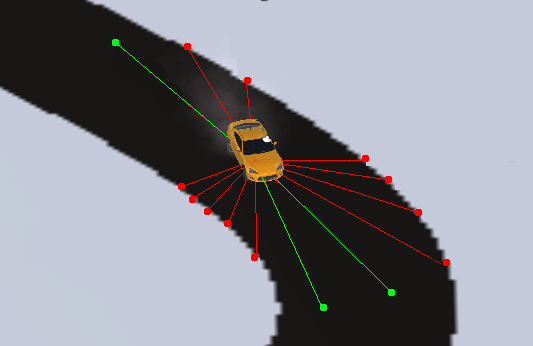
\includegraphics[width=.5\textwidth]{figures/observations_0}
    \caption{Obserwacje bota dystansów na około pojazdu}
    \label{fig}
\end{figure}
Dodatkowo przekazywana jest aktualna prędkość pojazdu jako obserwacja, zważywszy że nie da się jej w żaden sposób odczytać z jednej klatki pomiarów.

\subsubsection{Dane wizualne jednowymiarowe}
Poniższe podejście testuje metodę obserwacji wykorzystującą bodźce wizualne. W tym przypadku tworzona jest lista wartości kolorów dla każdego punktu w stałej odległości od pojazdu. Generuje to okrąg kolorów na około pojazdu, który powinien być w stanie przekazać takie informacje jak zakręty na trasie, będąc znacznie mniejszego rozmiaru niż obraz z kamery. Na rysunku zaznaczono kilka promieni pobierających kolory otoczenia.
\begin{figure}[H]
    \centering
    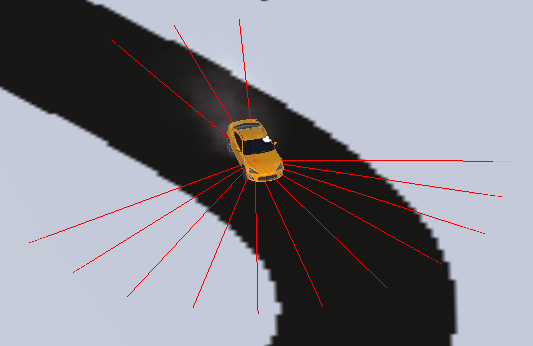
\includegraphics[width=.5\textwidth]{figures/observations_1}
    \caption{Obserwacje bota kolorów na około pojazdu}
    \label{fig}
\end{figure}
Dodatkowo przekazywana jest aktualna prędkość pojazdu jako obserwacja, zważywszy że nie da się jej w żaden sposób odczytać z danych wizualnych.

\subsubsection{Dane wizualne z kamery przedniej}
Wykorzystująć imformacje w postaci w jakiej są one widoczne dla każdego gracza, kolejna metoda pobiera obraz z kamery jako obserwacje. Kamera umiejscowiona jest na przedzie pojazdu, zapewniając perspektywę podobną do zwykłego prowadzenia auta. Aby ograniczyć ilość informacji dostarczanych do sieci, obraz z kamery skalowany jest do rozdzielczości $40x20$ oraz konwertowany na skalę szarości. Dodatkowo, jak powyżej, przekazywana jest aktualna prędkość pojazdu.
\begin{figure}[H]
    \centering
    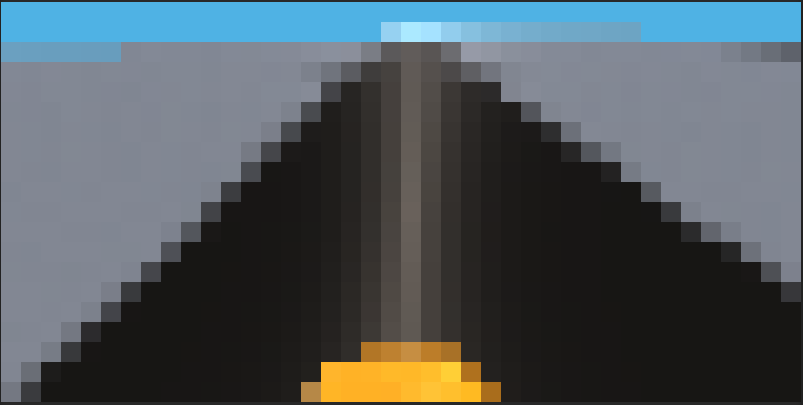
\includegraphics[width=.5\textwidth]{figures/observations_2}
    \caption{Obserwacje bota z kamery przedniej}
    \label{fig}
\end{figure}

\subsubsection{Dane wizualne z kamery z lotu ptaka}
Wykorzystująć imformacje widoczne przez kamerę z lotu ptaka model powinien być w stanie łatwiej zauważyć krzywiznę toru. Tak jak powyżej, obraz z kamery skalowany jest do rozdzielczości $30x20$ oraz konwertowany na skalę szarości, oraz przekazywana jest aktualna prędkość pojazdu.
\begin{figure}[H]
    \centering
    
\includegraphics[width=.5\textwidth]{figures/observations_3}
    \caption{Obserwacje bota z kamery z lotu ptaka}
    \label{fig}
\end{figure}

\subsubsection{Porównanie}
Poniżej znajdują się wykresy porównujące szybkość uczenia się w pierwszych 400 000 iteracjach. Wykres pierwszy pokazuje otrzymaną nagrodę za akcję, uśrednioną dla każdego agenta, dla każdej akcji. Drugi wykres przedstawia jak daleko udało się dojechać. Na przestrzeni całego toru rozłożone jest 40 punktów kontrolnych. Celem jest maksymalizacja obu wartości.
\begin{figure}[H]
    \centering
    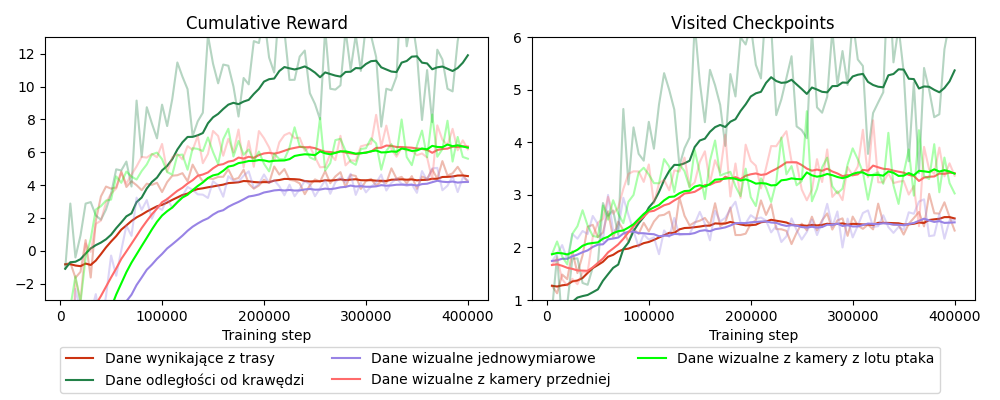
\includegraphics[width=\textwidth]{graphs/input_observations}
    \caption{Porównanie metod obserwacji}
    \label{fig}
\end{figure}
Najlepsze wyniki otrzymano dla metody wykorzystującej odległości od przeszkód. Metoda ta zbiera łącznie 14 dystansów, co wystarcza do zawarcia najpotrzebniejszych informacji. Dane z kamery okazały się zbyt obszerne (odpowiednio 600 i 800 pikseli), spowalniając trening.
\clearpage
\subsection{Wybór akcji}
Po podjęciu decyzji bot musi wykonać odpowiednią akcję. Bot podejmuje decyzję w dwóch płaszczyznach. Pierwsza odnosi się do przemieszczania przód-tył, natomiast dróga odpowiada skręceniu kierownicy prawo-lewo. Decyzje te mogłyby być wybierane z przestrzeni ciągłych lub dyskretnych.

\subsubsection{Akcje w przestrzeni ciągłej}
Dla każdej płaszczyzny bot zwraca wartość rzeczywistą z zakresu $[-1, 1]$. W pierwszej płaszczyźnie wartość odpowiada dokładnie stopniowi wciśnięcia pedału gazu, natomiast w drugiej - kątowi skrętu kierownicy. Poniważ bot jest w stanie zawsze ustawić konkretną wartość, przejścia pomiędzy kolejnymi akcjami nie muszą być płynne - w pierwszej klatce bot może skierować kierownicę 30 stopni w lewo, natomaist już klatkę później może ustawić ją na 20 stopni w prawo, bez stanów przejściowych.

\subsubsection{Akcje w przestrzeni dyskretnej}
Dla każdej płaszczyzny bot zwraca wartość całkowita ze zbioru ${-1, 0, 1}$. W pierwszej płaszczyźnie wartość $-1$ odpowiada zwiększeniu nacisku na pedał hamulca, $0$ oznacza brak zmian, $1$ oznacza zwiększenie nacisku na pedał gazu. Analogicznie w drugiej plaszczyźnie, $-1$ odpowiada skręceniu kierownicy mozniej w lewo, $1$ mocniej w prawo, a $0$ brak zmian. W ten sposób zmiany są bardziej płynne w czasie.

\subsubsection{Porównanie}
Zastosowanie akcji dyskretnych pozwoliło botowi na zancznie łatwiejsze poruszanie się w środowisku, co przełożyło sie na znacznie lepsze wyniki w pierwszych 400 000 krokach treningu.
\begin{figure}[H]
    \centering
    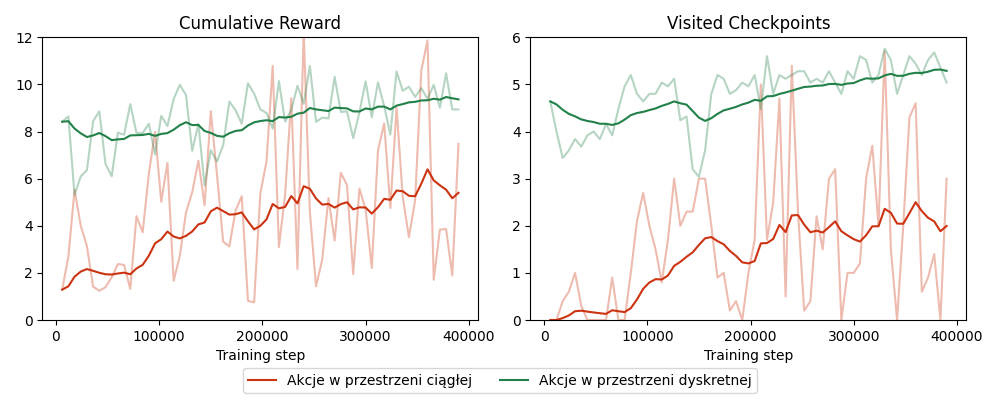
\includegraphics[width=\textwidth]{graphs/output_actions}
    \caption{Porównanie metod podejmowania akcji}
    \label{fig}
\end{figure}
\clearpage

\subsection{Zdefiniowanie funkcji oceny}
Ocena powinna odzwierciedlać w jakim stopniu wykonana akcja przybliżyła bota do osiągnięcia celu. W każdym cyklu, podjęta akcja oceniana jest na podstawie trzech parametrów.
\begin{align*}
    Q &= (0.5 - distanceToRoadCenter) \cdot 0.1 + \\
    & (0.05 - abs(angleToTangent)) + \\
    & (distanceTraveledInFrame - 0.1) + \\
    & 0.01
\end{align*}
Po pierwsze przyznawana jest nagroda za utrzymywanie sie w odległości mniejszej niż 50\% szerokości drogi od środka drogi (linia czerwona na poniższym rysunku), w przeciwnym przypadku kara, wprost proporcjonalna do ww. odległości. Po drugie przyznawana jest nagroda za utrzymywanie kierunku jazdy (linia zielona na poniższym rysunku) w zakresie $\pm10$ stopni od kierunku trasy (linia niebieska na poniższym rysunku), w przeciwnym przypadku kara, wprost proporcjonalna do w.w kąta. Po trzecie przyznawana jest nagroda za dystans pokonany od ostatniej akcji, jeżeli wynosi co najmniej $0.1$. Dodatkowo przyznawana jest nagroda za każdą klatkę, aby promować jak najdłuższe treningi.
\begin{figure}[H]
    \centering
    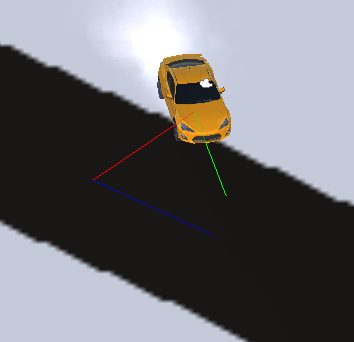
\includegraphics[width=.5\textwidth]{figures/rewards}
    \caption{Wizualizacja oceny akcji}
    \label{fig}
\end{figure}
Dodatkowo bot oceniany jest za każdym razem kiedy wejdzie w interakcję z innym obiektem. Na około całego terenu rozmieszczone są bariery, które powodują koniec epizodu po dotknięciu i powrót pojazdu na pozycję początkową, dodatkowo dodając karę $0.1$. Na pierwszym etapie treningu takie same bariery ustawione są wzdłuż drogi, tak że pojazd kończy epizod za każdym razem kiedy zjedzie z drogi. Po wytrenowaniu bota w takich warunkach bariery te zostaną ściągnięte, aby zobaczyć czy mimo to bot będzie trzymał sie drogi.\\
Wzdłuż całej trasy rozstawione są punkty kontrolne, które pojazd powinien przebyć w odpowiedniej kolejności. Za każdy punkt kontrolny zaliczony w kolejności nagroda zwiększa się o $1$. Jeżeli pojazd zahaczy o któryś z 4 sąsiednich punktów kontrolnych (2 w tył, 2 w przód) dostaje tylko karę $0.1$, natomiast jeżeli dotknie innego punktu kontrolnego, epizod jest kończony z karą $-1$.
\begin{figure}[H]
    \centering
    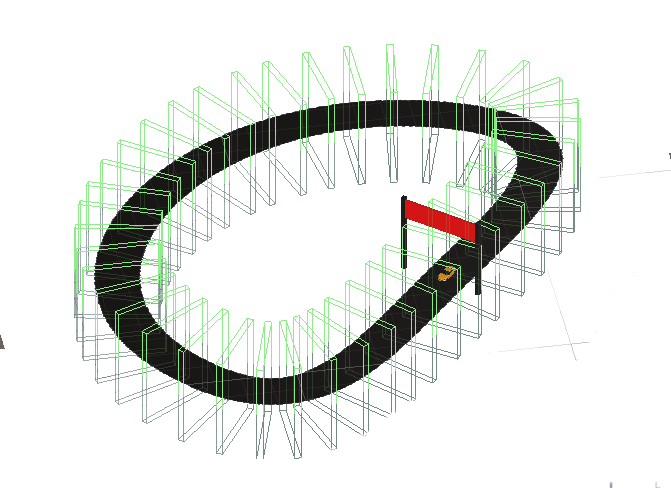
\includegraphics[width=.5\textwidth]{figures/checkpoints}
    \caption{Rozmieszczenie punktów kontrolnych}
    \label{fig}
\end{figure}

\subsection{Dobranie parametrów}
Wybrany algorytm Proximal Policy Optimization pozwala na osiągnięcie nie najgorszych wyników, natomiast dostosowanie hyperparametrów potrafi znacznie poprawić efekty treningu.
\\\\
\begin{algorithm}[H]
\caption{Hiperparametry początkowe treningu}\label{alg}
$hyperparameters:$\\
    \hskip2em $batch\_size: 1024$\\
    \hskip2em $buffer\_size: 10240$\\
    \hskip2em $learning\_rate: 0.0003$\\
    \hskip2em $beta: 0.005$\\
    \hskip2em $epsilon: 0.2$\\
    \hskip2em $lambd: 0.95$\\
    \hskip2em $num\_epoch: 3$\\
    \hskip2em $learning\_rate\_schedule: linear$\\
% $network\_settings:$\\
%     \hskip2em $normalize: False$\\
%     \hskip2em $hidden\_units: 128$\\
%     \hskip2em $num\_layers: 2$\\
%     \hskip2em $vis\_encode\_type: simple$\\
%     \hskip2em $memory: None$\\
%     \hskip2em $goal\_conditioning\_type: hyper$\\
$reward\_signals:$\\
    \hskip2em $extrinsic:$\\
        \hskip4em $gamma: 0.99$\\
        \hskip4em $strength: 1.0$\\
\end{algorithm}
\phantom{.}\\
Poniżej zostały przedstawione wybory poszczególnych parametrów. Porównane zostały konfiguracje dla pierwszych $500 000$ iteracji, za każdym razem zaczynając od losowych wag. Po wyborze optymalnej wartości parametru, była ona aktualizowana i wykorzystywana w kolejnych testach jako domyślna.\\
\clearpage

\subsection{gamma}
Parametr $gamma$ można rozumieć jako jak daleko w przyszłość agent powinien dbać o możliwe nagrody. W sytuacjach gdy agent powinien podejmować decyzje w oczekiwaniu na przewidywane nagrody w przyszłości, wartość $gamma$ powinna być większa ($0.995$), natomiast jeżeli agent powinien bardziej dbać o nagrody natychmiastowe wartość $gamma$ może osiągać niższe wartości ($0.8$). Po porównaniu granic typowego zakresu wartości, na wykresach poniżej widać, że wartość niższa przekłada się na minimalnie lepszy trening.
\begin{figure}[H]
    \centering
    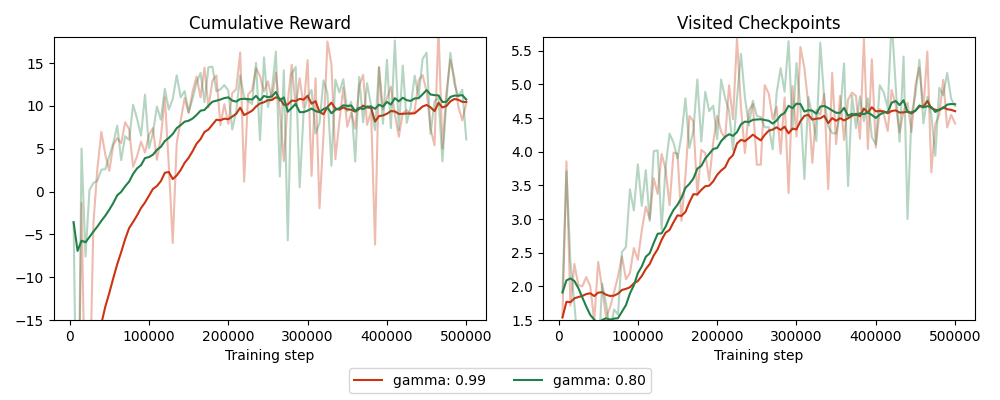
\includegraphics[width=\textwidth]{graphs/hyperparameters_gamma.png}
    \caption{Wybór hiperparametrów: gamma}
    \label{fig}
\end{figure}

\subsection{lambda}
Parametr $lambda$ definiuje w jakim stopniu agent polega na przewidzianej wartości podczas przewidywania kolejnej wartości. Niższe wartości $lambda$ oznaczają poleganie w większym stopniu na przewidzianej wartości, natomiast większa $lambda$ odpowiada poleganiu bardziej na rzeczywiście otrzymanych nagrodach. Po porównaniu granic typowego zakresu wartości ($0.85-0.95$), na wykresach poniżej widać, że wartość niższa przekłada się na minimalnie lepszy trening.
\begin{figure}[H]
    \centering
    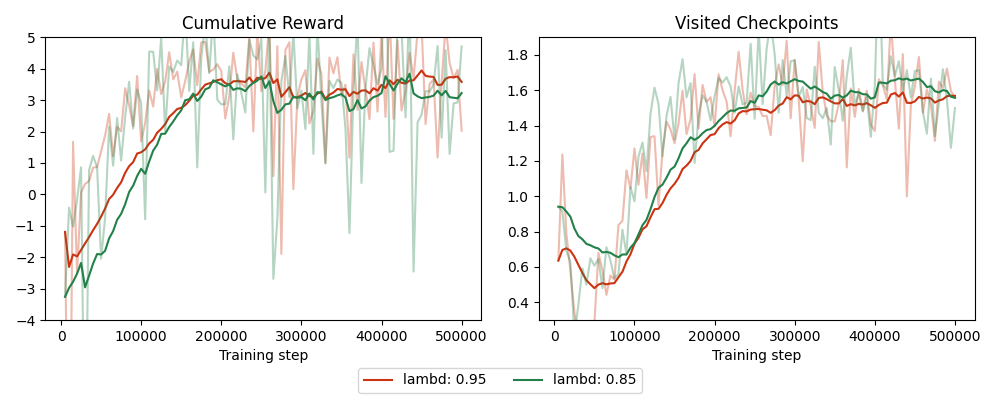
\includegraphics[width=\textwidth]{graphs/hyperparameters_lambd.png}
    \caption{Wybór hiperparametrów: lambd}
    \label{fig}
\end{figure}

\subsection{buffer size}
Rozmiar bufora odpowiada ilości cykli treningowych (zebranie obserwacji, podjęcie akcji, otrzymanie nagrody) które są zbierane przed aktualizacją modelu. Większa wartość przekłada się na bardziej stabilny trening, kosztem czasu. Po porównaniu wartości $10240$ i $40960$ można zauważyć, że niższa wartość zapewnia zadowalającą stabilność, otrzymując podobne wartości znacznie wcześniej.
\begin{figure}[H]
    \centering
    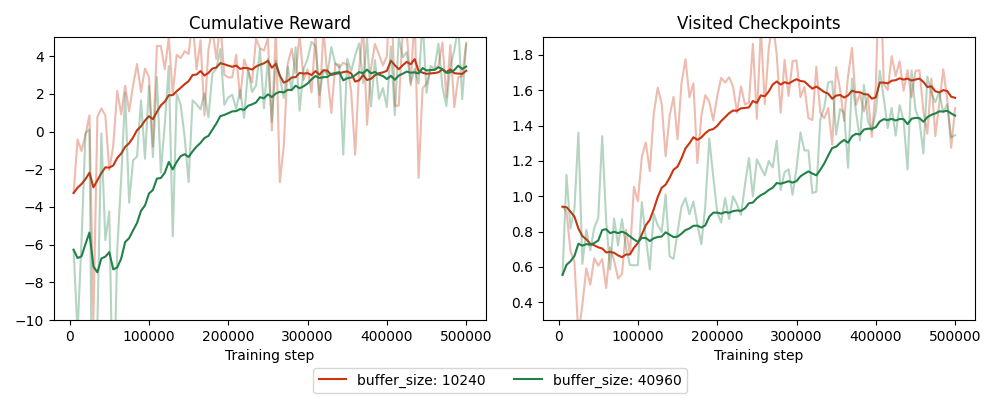
\includegraphics[width=\textwidth]{graphs/hyperparameters_buffer_size.png}
    \caption{Wybór hiperparametrów: buffer size}
    \label{fig}
\end{figure}

\subsection{batch size}
Parametr $batch\_size$ definiuje ilość cykli treningowych wykorzystywanych przy propagacji wstecznej. Przy dyskretnej przestrzeni akcji wartość ta powinna być mniejsza, niż dla akcji ciągłych. Zmniejszenie $batch\_size$ do $256$ minimalnie poprawiło trening, natomiast spadek do $32$ nie wprowadził zauważalnych różnic.
\begin{figure}[H]
    \centering
    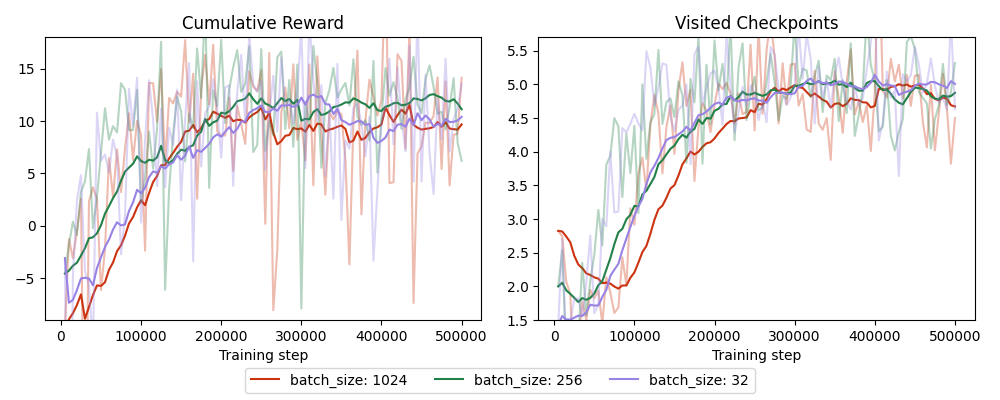
\includegraphics[width=\textwidth]{graphs/hyperparameters_batch_size.png}
    \caption{Wybór hiperparametrów: batch size}
    \label{fig}
\end{figure}
\clearpage

\subsection{learning rate}
Prędkość uczenia bezpośrednio odnosi się do siły każdego kroku propagacji wstecznej. Analizując poniższe wykresy, wartość pośrodku typowego zakresu ($1e-3, 1e-5$) pozwala na najbardziej optymalną prędkość uczenia w skali 500000 iteracji.
\begin{figure}[H]
    \centering
    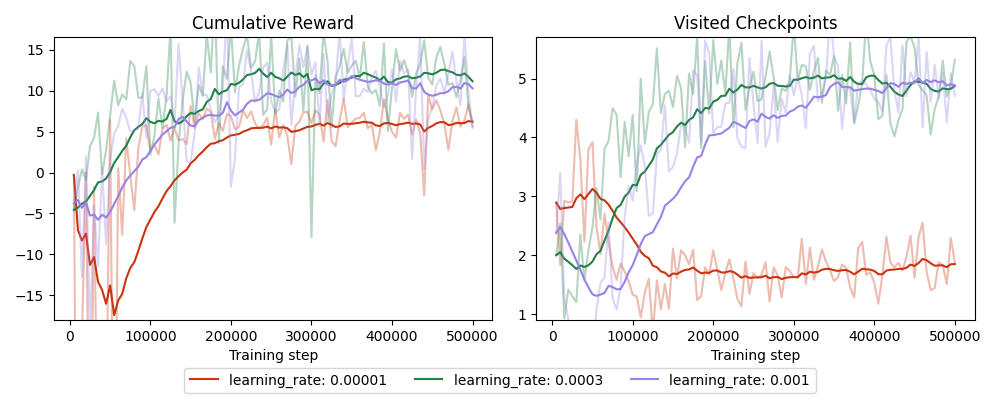
\includegraphics[width=\textwidth]{graphs/hyperparameters_learning_rate.png}
    \caption{Wybór hiperparametrów: learning rate}
    \label{fig}
\end{figure}

\subsection{beta}
Parametr $beta$ definiuje skalę randomizacji polityki. Większe wartości parametru powodują podejmowanie przez bota większej ilości losowych akcji, zwiększając ilość sprawdzanych rozwiązań. Dla zadanego problemu niższa $beta$ powoduje szybsze unormowanie się wartości nagrody oraz postępu trasy, dlatego została wybrana wartość $0.005$.
\begin{figure}[H]
    \centering
    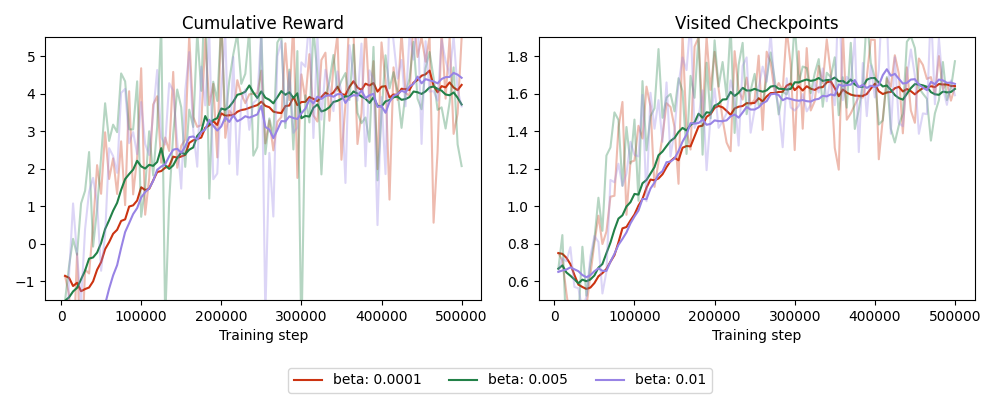
\includegraphics[width=\textwidth]{graphs/hyperparameters_beta.png}
    \caption{Wybór hiperparametrów: beta}
    \label{fig}
\end{figure}
\clearpage

\subsection{epsilon}
Zmienna $epsilon$ informuje w jakim stopniu akceptowane są rozbieżności pomiędzy starą i nową polityką podczas propagacji wstecznej. Niższe wartości powodują bardziej stabilny postęp kosztem czasu treningu. Zwiększenie wartości do $0.4$ nie spowodowało jednak przyspieszenia treningu.
\begin{figure}[H]
    \centering
    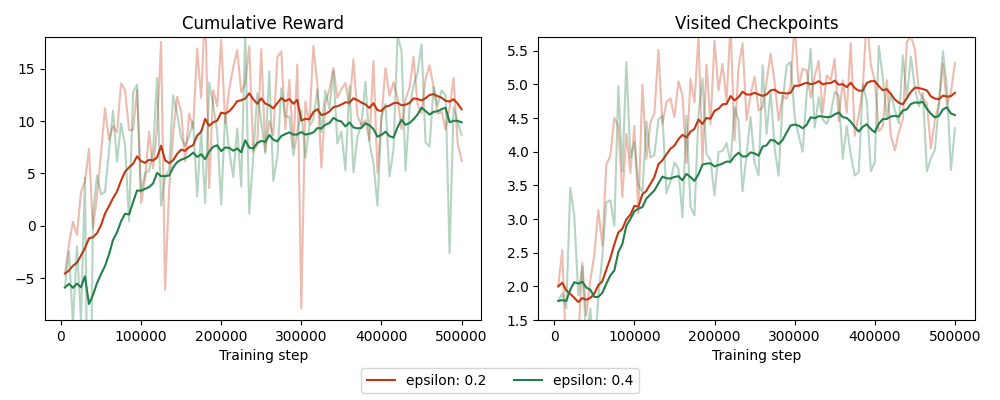
\includegraphics[width=\textwidth]{graphs/hyperparameters_epsilon.png}
    \caption{Wybór hiperparametrów: epsilon}
    \label{fig}
\end{figure}

% \subsection{visual encode type}
% Ponieważ agent korzysta z danych wizualnych z kamery, są one procesowane przez konwolucyjną sieć neuronową. Poniżej zostały porównane trzy rodzaje sieci konwolucyjnych z prostą siecią łączącą wszystkie wejścia z wszystkimi wyjściami (\textit{fully connected}). Sieć $simple$ składa się tylko z dwóch warstw konwolucyjnych. Sieć $resnet$ wykorzystuje znacznie większą implementację IMPALA Resnet \cite{ImpalaResnet}. Sieć $match3$ \cite{Match3} jest mniejszą siecią konwolucyjną zoptymalizowaną dla gier planszowych i o segmentowym układzie, co dobrze reaguje na wykorzystanie kamery niskiej rozdzielczości, gdzie każdemu pikselowi odpowiada komórka gry.
% \begin{figure}[H]
%     \centering
%     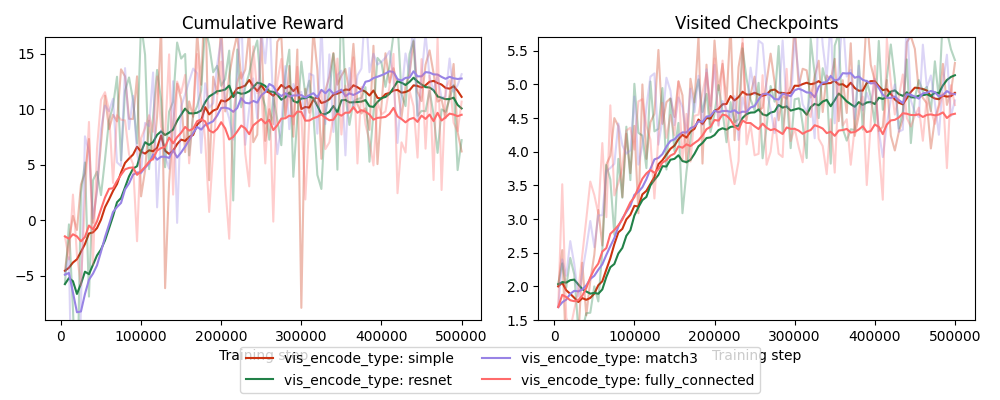
\includegraphics[width=\textwidth]{graphs/hyperparameters_vis_encode_type.png}
%     \caption{Wybór hiperparametrów: vis encode type}
%     \label{fig}
% \end{figure}

% \subsection{network size}
% \begin{figure}[H]
    %     \centering
    %     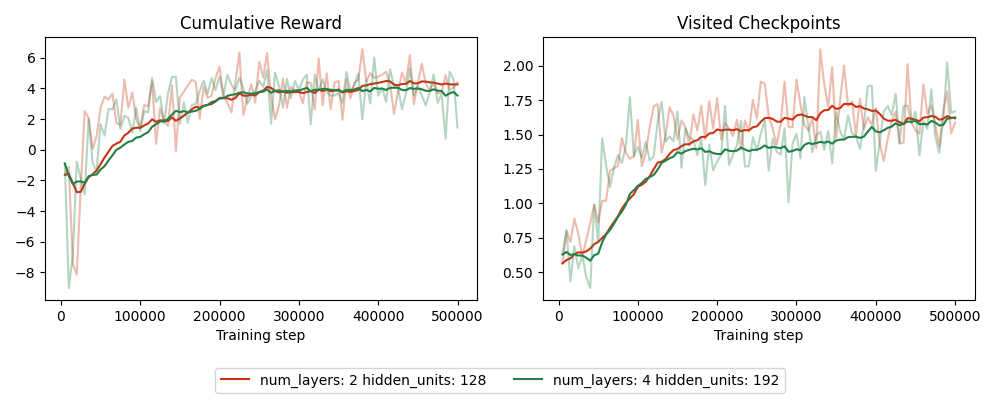
\includegraphics[width=\textwidth]{graphs/hyperparameters_network_size.png}
    %     \caption{Wybór hiperparametrów: layers, hidden units}
    %     \label{fig}
    % \end{figure}

Finalnie zostały wybrane poniższe hiperparametry, co pozwoliło na zauważalną poprawę treningu. Średnia wartość nagrody dla całego okresu wzrosła z $2.46$ do $3.26$ ($+32.5\%$), natomaist stopień postępu trasy wzrósł z $1.305$ do $1.499$ ($+14.9\%$).
\begin{figure}[H]
    \centering
    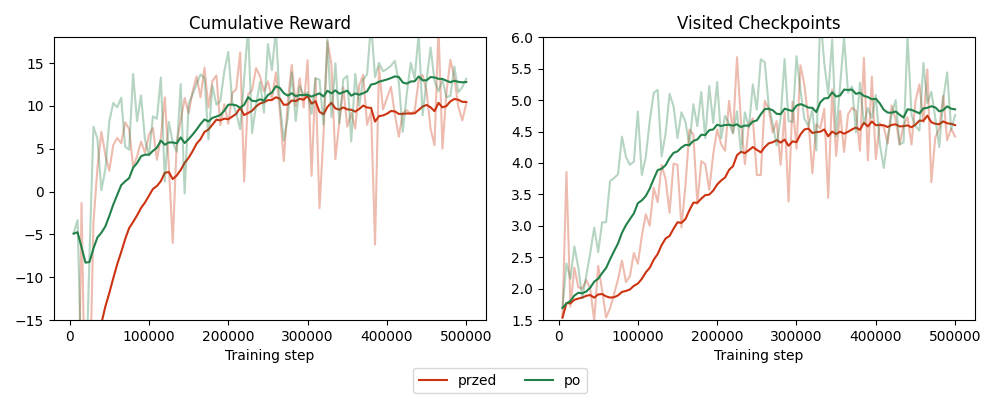
\includegraphics[width=\textwidth]{graphs/hyperparameters_tuning_results.png}
    \caption{Wybór hiperparametrów: porównanie wyników}
    \label{fig}
\end{figure}
\begin{algorithm}[H]
\caption{Hiperparametry finalne treningu}\label{alg}
$hyperparameters:$\\
    \hskip2em $batch\_size: 256$\\
    \hskip2em $buffer\_size: 10240$\\
    \hskip2em $learning\_rate: 0.0003$\\
    \hskip2em $beta: 0.005$\\
    \hskip2em $epsilon: 0.2$\\
    \hskip2em $lambd: 0.85$\\
    \hskip2em $num\_epoch: 8$\\
    \hskip2em $learning\_rate\_schedule: linear$\\
% $network\_settings:$\\
%     \hskip2em $normalize: False$\\
%     \hskip2em $hidden\_units: 128$\\
%     \hskip2em $num\_layers: 2$\\
%     \hskip2em $vis\_encode\_type: match3$\\
%     \hskip2em $memory: None$\\
%     \hskip2em $goal\_conditioning\_type: hyper$\\
$reward\_signals:$\\
    \hskip2em $extrinsic:$\\
        \hskip4em $gamma: 0.8$\\
        \hskip4em $strength: 1.0$\\
\end{algorithm}
\clearpage
\subsection{Dalsze etapy treningu}
Przy trenowaniu ważne jest, aby początkowe zadania były proste, aby agent był w stanie je łatwo wykonać. Następnie należy stopniowo zwiększać poziom trudności, dając agentowi odpowiednio dużo czasu na przystosowanie się do zmian. Dlatego pierwszy etap treningu polega na przejechaniu trasy będącej okręgiem, po płaskim terenie, bez wykorzystania tekstur (droga jest czarna, otoczenie białe) oraz bez przeciwników (w każdym środowisku znajduje się jeden agent).
\begin{figure}[H]
    \centering
    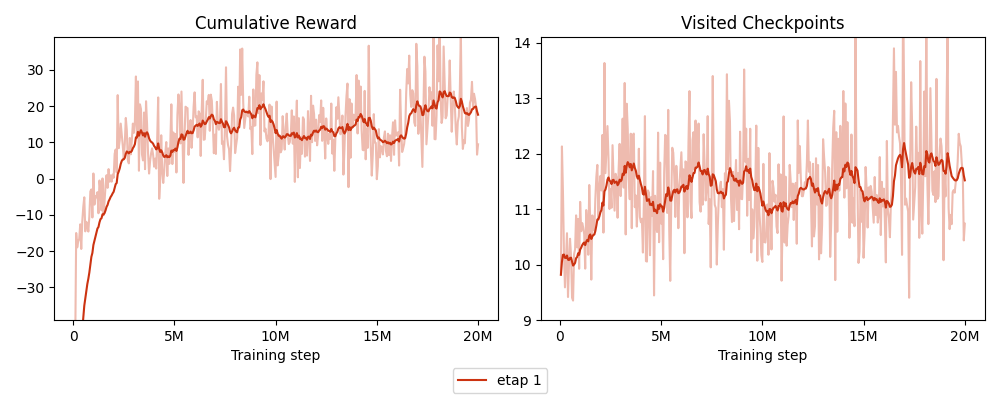
\includegraphics[width=\textwidth]{graphs/training_progress_1.png}
    \caption{Postep treningu: etap 1}
    \label{fig}
\end{figure}
\phantom{.}\\
Etap 2 zakłada dodanie większej różnorodności torów, zachowując stosunkowo prosty kształt, tylko nieznacznie odbiegający od okręgu, z małą ilością ostrych zakrętów.\\
% \textbf{TODO wykres postępu}\\
Etap 3 sprawdza adaptowalność pojazdu na skomplikowanym torze, z dużą ilością ostrych zakrętów.\\
% \textbf{TODO wykres postępu}\\
Etap 4 zakłada dodanie nierówności terenu, tworząc góry i pagórki na trasie.\\
% \textbf{TODO wykres postępu}\\
